\section{Model}
\label{sec:model}

\subsection{Preliminaries}
\label{sec:model:prelim}

Following the SQL:2011
standard~\cite{DBLP:journals/sigmod/KulkarniM12}, we adopt the {\em
  closed-open} period model, where a period (or interval) represents a
continuous set of time instances, starting from and including the
start time, continuing to but excluding the end time.

\begin{definition}[Time period]
A {\em time period} \\$p = [start, end)$ is an interval of the
  continuous time domain, subject to the constraint $start < end$.
\label{def:period} 
\end{definition}

It will be useful to quantify relationships between time periods using
the following Allen's relations~\cite{allen83} with equality:
\predName{meets}, \predName{overlaps}, \predName{starts},
\predName{finishes}, \predName{during}, and \predName{equals}.  We
will use $\pred{p}{contains}{q}$ as a shorthand for
$\pred{p}{starts}{q} \vee \pred{p}{finishes}{q} \vee
\pred{p}{during}{q} \vee \pred{p}{equal}{q}$.

We will use $p \cap q$ to denote the intersection of time periods $p$
and $q$: $[\predName{max}(p.start,q.start), \predName{min}(p.end,
  q.end))$.

\begin{figure}
\centering
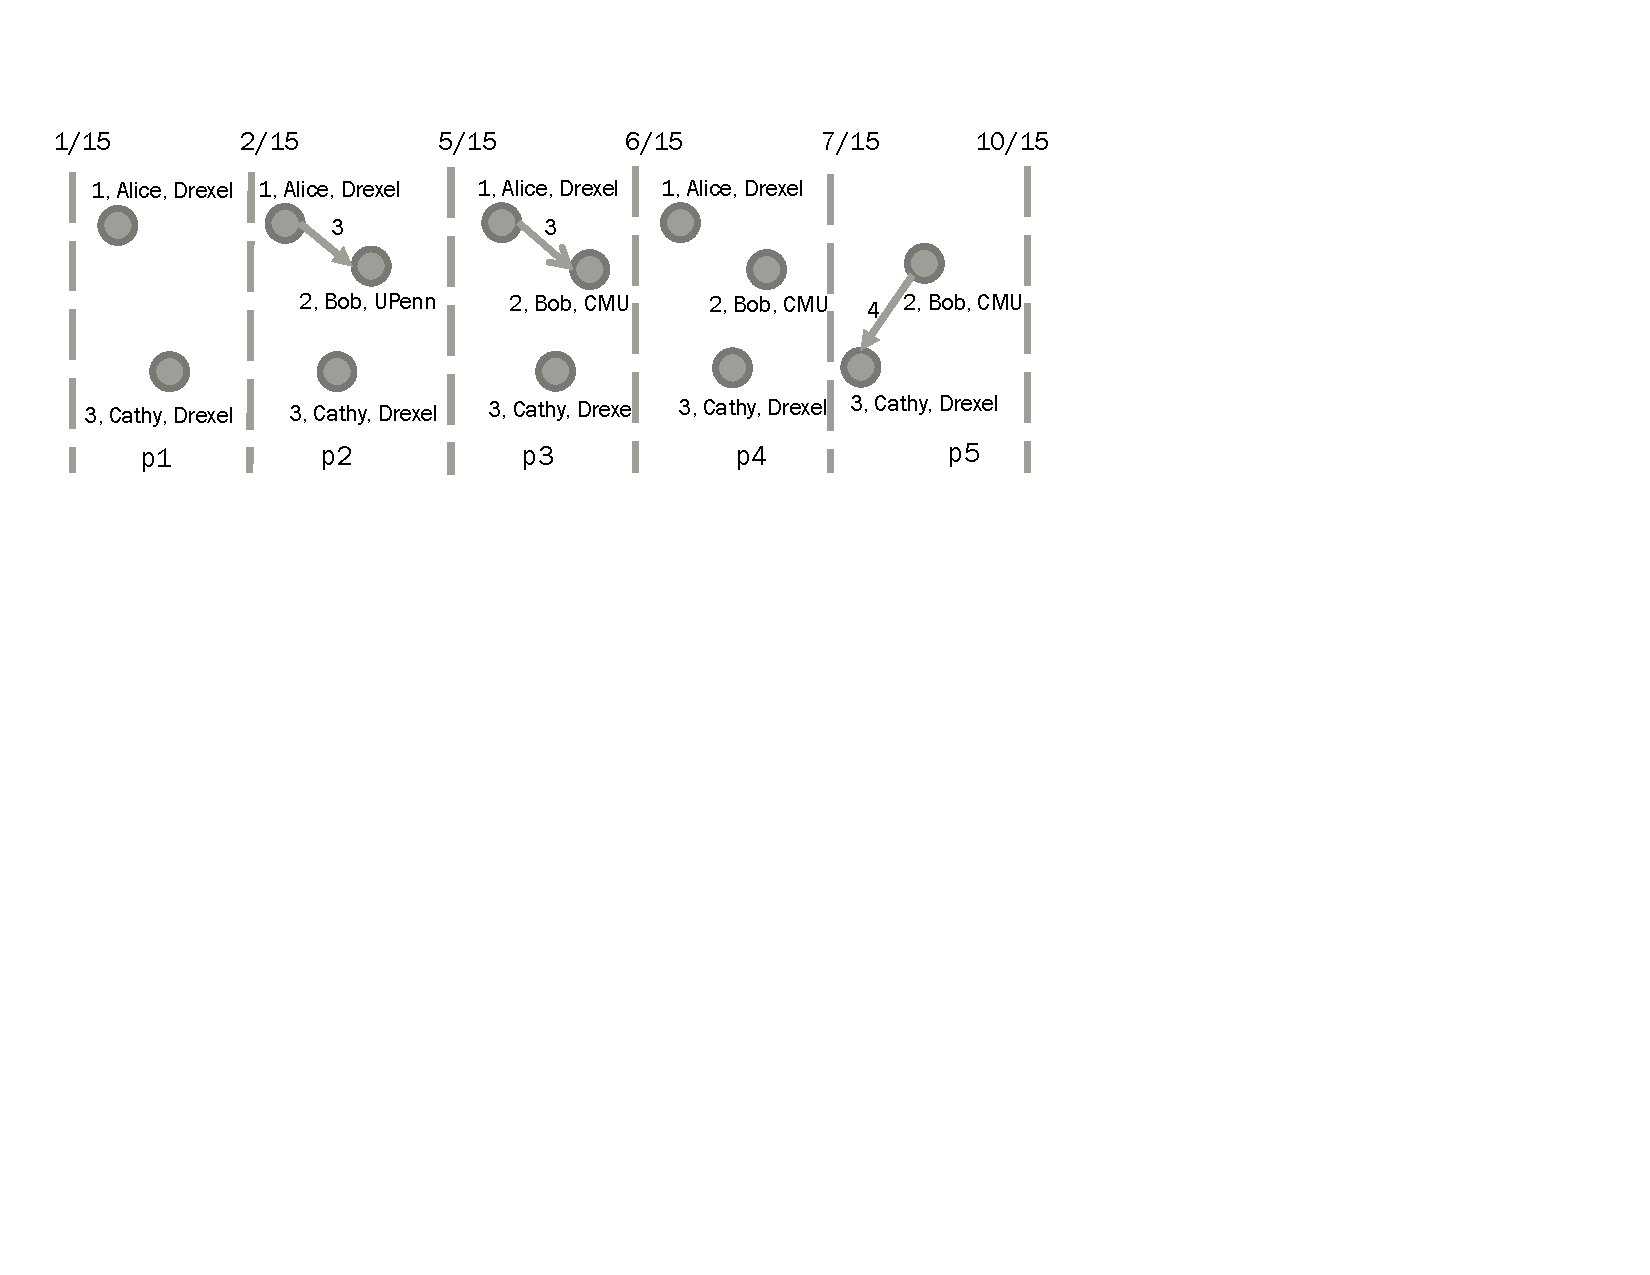
\includegraphics[width=3.5in]{figs/T1_graphs.pdf}
\caption{Representative graphs of \tg \insql{T1}.}
\label{fig:tg_rg}
\end{figure}

\begin{figure}
\centering
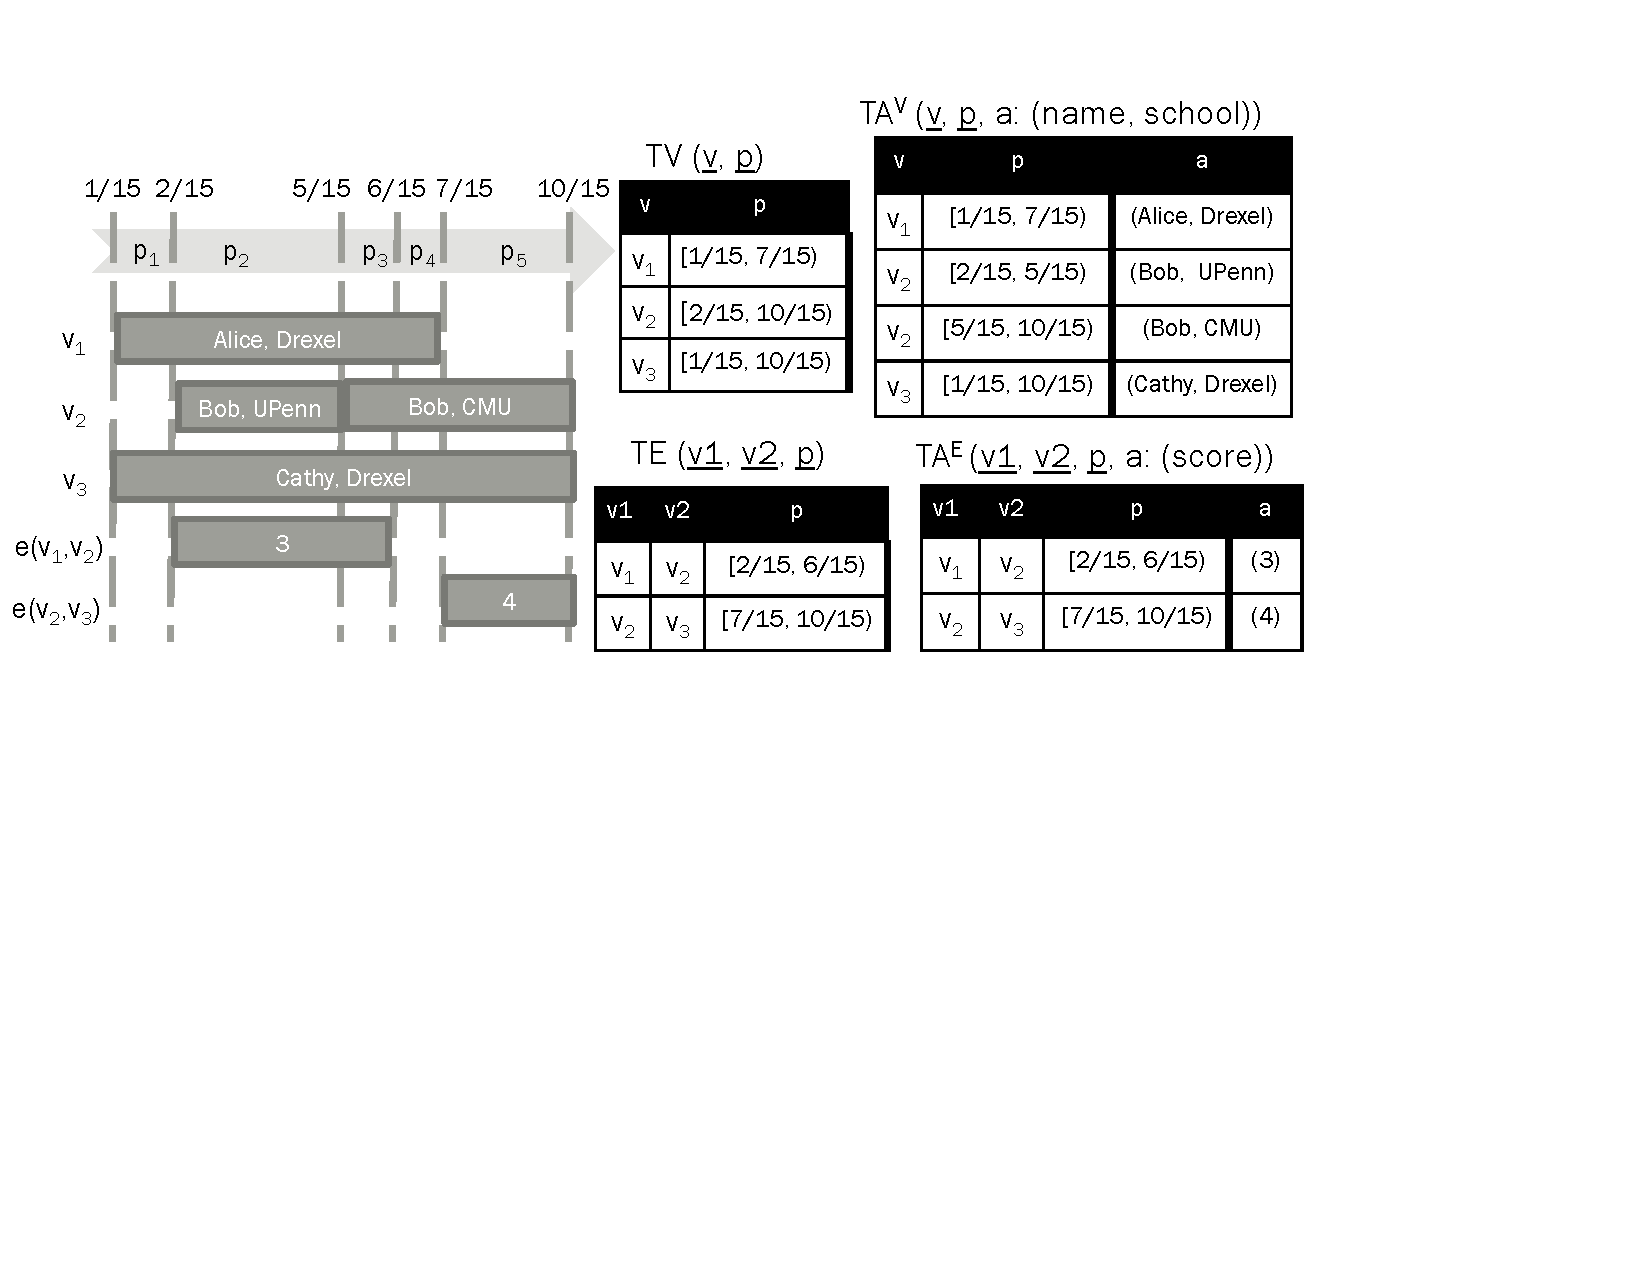
\includegraphics[width=3.5in]{figs/T1_rel_tab.pdf}
\caption{Vertex-edge representation of \tg
  \insql{T1}.}
\label{fig:tg_ve}
\end{figure}

\eat{It will be useful to quantify relationships between time periods $p$
and $q$ using the following Allen's relations~\cite{allen83}.}

\eat{\begin{itemize}
\item $p equal q$, defined as $p.start = q.start \wedge p.end = q.end$
\item $p overlaps q$, defined as $p.end > q.start$
\item $p meets q$, defined as $p.end = q.start$
\item $p during q$, defines as $p.start > q.start \wedge p.end < q.end$ 
\item $p starts q$, defined as $p.start = q.start \wedge p.end < q.end$
\item $p finishes q$, defined as $p.start > q.start \wedge p.end = q.end$
\end{itemize}}

\subsection{Representative graphs of a \tg}
\label{sec:model:rg}

The basic building block of our model is a \tg, which represents a
graph that evolves continuously over time, and is defined over a set
of vertices $V$, a set of edges $E\subseteq V \times V$, a set of
vertex labels \avv, and a set of edge labels \aee.

\begin{definition}[TGraph]
A \tg $\tgg(g, p)$ is a valid-time period-based relation in which a
tuple associates a state of the graph $g$ with a time period $p$
during which the graph is in that state.
%
Each $g = (V_g, E_g, \avv_g, \aee_g)$, with $V_g \subseteq V$, $E_g
\subseteq E$, $\avv_g \subseteq \avv$, $\aee_g \subseteq \aee$.
%
\tgg is temporally coalesced:
\begin{multline}
\forall \tgg(g,p)~~\nexists \tgg(g,p')~~| \\
        \pred{p}{meets}{p'}~\lor~\pred{p}{contains}{p'}~\lor~\pred{p}{overlaps}{p'}
\end{multline}
We refer to each $g$ that appears in some tuple $(g,p)$ of \tgg as a
representative graph of \tgg during period $p$.
\label{def:tg_abstract}
\end{definition}

An example of a \tg is given in Figure~\ref{fig:tg_rg}, where 5
representative graphs (states) of \insql{T1} are associated with 5
consecutive time periods $p_1=[1/15, 2/15), \ldots, p_5=[7/15, 10/15)$.
    Note that it is not required that time periods of a \tg be
    consecutive and with no gaps.

    Vertices and edges of a \tg are not required to be homogeneous in
    terms of their schemas.  In line with, e.g., Neo4j and GraphX,
    representative graphs use the property graph data
    model~\cite{GraphDB}.  That is, each vertex (resp. edge) of $g$
    during period $p$ has a collection of properties defined by a map
    from property name to value.

As is typically the case in interval-based models, each representative
graph is assumed to exists continuously, and remains unchanged, during
the associated period.  By this we mean that graph topology (identies
of its vertices and edges), and properties of each vertex and edge
remain unchanged.
%
The statement that \tgg is temporally coalesced means that each fact
(which in our case corresponds to unchanging state of the graph) is
represented exactly once for each time period of maximal length when
it holds~\cite{DBLP:conf/vldb/BohlenSS96}.\eat{ This is the standard
  meaning of the term ``coalesce'' in temporal databases, and is
  unrelated to the SQL coalesce function.}  For interval-based models,
requiring that relations be coalesced is both space-efficient and
avoids semantic ambiguity (see~\cite{DBLP:reference/db/JensenS09k}
Fig. 2 and its description).

\subsection{Vertex-edge representation of a \tg}
\label{sec:model:ve}

We now give an alternative representation of a \tg that uses
valid-time temporal SQL relations~\cite{DBLP:conf/vldb/BohlenSS96},
with nesting, to represent evolution of graph topology and of its
vertex and edge attributes (both schemas and values).  We term this
logical representation the {\em \ve \tg}.  An example of a \ve \tg is
given in Figure~\ref{fig:tg_ve}.  We will refer to the \rgs
(Definition~\ref{def:tg_abstract}) and \ve (Definition~\ref{def:tg})
represenations of a \tg jointly as \insql{T}, and will disambiguate
between the two representations with \trg and \tve when necessary.

\eat{ Following notation in~\ref{DBLP:conf/vldb/BohlenSS96}, we will
  make use of $value\_equivalent(x,y) = (x[A] = y[A])$ --- a Boolean
  predicate that evaluates to true of $x$ and $y$ agree on values of
  their explicit (non-temporal) attributes.}

\begin{definition}[Vertex-Edge TGraph]
A vertex-\\edge representation of \tg is a pair $\tve=(\tv, \te)$. \tv
is a valid-time temporal SQL relation with schema $\tv(\underline{v},
\underline{p})$, in which a tuple associates a vertex with the time
period during which it was present. \te is a valid-time temporal SQL
relation with schema $\te(\underline{v_1}, \underline{v_2},
\underline{p})$, connecting pairs of vertices from \tv.  Attribute $p$
represents time period (as per Definition~\ref{def:period}).  Both \tv
and \te are coalesced:

\begin{multline}
\forall \tv(v, p)~~\nexists \tv(v, p')~~| \\
                       \pred{p}{meets}{p'}~\lor~\pred{p}{contains}{p'}~\lor~\pred{p}{overlaps}{p'}
\label{def:tg:c2}
\end{multline}
\vspace{-0.5cm}
\begin{multline}
\forall \te(v_1, v_2, p)~~\nexists \te(v_1,v_2, p')~~| \\
                       \pred{p}{meets}{p'}~\lor~\pred{p}{contains}{p'}~\lor~\pred{p}{overlaps}{p'}
\label{def:tg:c3}
\end{multline}

An edge connects a pair of vertices that exist at the time when the edge exists:
\begin{multline}
\forall \te(v_1, v_2, p)~~\exists \tv(v_1, p_1), \tv(v_2, p_2)~~| \\
                       \pred{p_1}{contains}{p}~\wedge~\pred{p_2}{contains}{p}
\label{def:tg:c1}
\end{multline}
\vspace{-0.5cm}

\insql{T} optionally includes a vertex attribute relation \tav and an
edge attribute relation \tae.  \tav is coalesced, and associates
attribute values (properties) with existing vertices.
\begin{multline}
\forall \tav(v, p, a)~~\nexists \tav(v, p', a)~~| \\
                       \pred{p}{meets}{p'}~\lor~\pred{p}{contains}{p'}~\lor~\pred{p}{overlaps}{p'}
\label{def:tg:c4}
\end{multline}
\begin{multline}
\forall \tav(v, p, a)~~\exists \tv(v,p')~~|~~\pred{p'}{contains}{p}
\label{def:tg:c5}
\end{multline}
\tae is coalesced, and associates attribute values (properties) with
existing edges.
\begin{multline}
\forall \tae(v_1, v_2, p, a)~~\nexists \tae(v_1, v_2, p', a)~~| \\
                       \pred{p}{meets}{p'}~\lor~\pred{p}{contains}{p'}~\lor~\pred{p}{overlaps}{p'}
\label{def:tg:c6}
\end{multline}
\begin{multline}
\forall \tae(v_1, v_2, p, a)~~\exists \te(v_1,v_2,p')~~|~~\pred{p'}{contains}{p}
\label{def:tg:c7}
\end{multline}

\label{def:tg}
\end{definition}

Graphs may be directed or undirected.  For undirected graphs we choose
a canonical representation of an edge, with $v_1 \leq v_2$ (self-loops
are allowed).

Conditions~\ref{def:tg:c2} and~\ref{def:tg:c3} in
Definition~\ref{def:tg} state that \tv and \te are
coalesced~\cite{DBLP:conf/vldb/BohlenSS96}, i.e., that each vertex and
edge is represented exactly once for each time period of maximal
length when it is present.  Conditions~\ref{def:tg:c4}
and~\ref{def:tg:c6} state that all attribute relations are coalesced,
i.e., that an attribute is represented exactly once for each time
period of maximal length in which its value did not change.  Consider
\insql{T1} in Figure~\ref{fig:tg_ve} and note that there is a single
tuple corresponding to vertex $v_2$ in \tv, but two tuples
corresponding to $v_2$ in \tav, because the value of $a.school$
changed at time $t_2$.

Definitions~\ref{def:tg_abstract} and~\ref{def:tg} give two
alternative views of graph evolution.  In
Definition~\ref{def:tg_abstract} the graph is represented in its
entirety, with a change of state occurring whenever there is a change
in graph topology or in its vertex or edge properties.  In other
words, time periods here are at their finest granularity.  In
contrast, Definition~\ref{def:tg} decouples evolution of graph
vertices, edges and attribute values, coalescing each relation
independently of the others.  This makes graph maintenance and
manipulation more manageable.

The \tv and \te relations of Definition~\ref{def:tg}, although only
partially enforcing the constraints, can be implemented as follows (as
per SQL:2011):

\eat{ Condition~\ref{def:tg:c1} in Definition~\ref{def:tg} states the
  natural integrity constraint that an edge linking two vertices can
  only exist during a time when both vertices exist. Here,
  $\pred{p}{contains}{q}$ is the Allen \predName{contains} relation
  with equality~\cite{allen83}, defined as $p.start \leq q.start
  \wedge p.end \geq q.end$.  Consider the vertex-edge representation
  of \tg \insql{T1} in Figure~\ref{fig:tg_ve}, where edge $e(v_1,v_2)$
  exists during the entire period when both $v_1$ and $v_2$ exist,
  while edge $e(v_2,v_3)$ exists only for a portion of the period when
  both $v_2$ and $v_3$ exist.}

\begin{small}
\begin{verbatim}
CREATE TABLE TV (
  v LONG,
  pstart DATE,
  pend DATE,
  PERIOD for p (pstart, pend),
  PRIMARY KEY (v, p WITHOUT OVERLAPS) )

CREATE TABLE TE (
  v1 LONG,
  v2 LONG,
  pstart DATE,
  pend DATE,
  PERIOD for p (pstart, pend),
  PRIMARY KEY (v1, v2, p WITHOUT OVERLAPS),
  FOREIGN KEY (v1, PERIOD p) REFERENCES TV(v, PERIOD p),
  FOREIGN KEY (v2, PERIOD p) REFERENCES TV(v, PERIOD p) )
\end{verbatim}
\end{small}

Unfortunately, this implementation does not guarantee that \tv and \te
will be coalesced.  It does ensure that time periods corresponding to
a vertex (resp. edge) do not overlap, and that one does not contain
the other, but it does not prevent the existence of two adjacent time
periods for a vertex or edge, i.e., periods $p$ and $q$ for which
$\pred{p}{meets}{q}$.  That is, there may well be two tuples in \tv
for $v_1$ in Figure~\ref{fig:tg_ve}, one associated with $[1/15,
  2/15)$ and the other with $[2/15, 7/15)$.

Temporal SQL, as per the SQL:2011 standard, (1) does not provide a way
to specify that a relation be coalesced, and (2) does not enable
efficient mechanisms to implement the coalesce operator.  Coalescing
requires that the system automatically merge adjacent and overlapping
time periods.  This operation, which is similar to duplicate
elimination in conventional databases, has been extensively studied in
the
literature~\cite{DBLP:conf/vldb/BohlenSS96,DBLP:journals/sigmod/Zimanyi06},
but is not supported by the standard.  Note that, while it is an
important property of our logical model that time periods be
coalesced, eagerly coalescing is both expensive and, in some cases,
unnecessary.  We will discuss this when presenting \tg algebra
(Section~\ref{sec:algebra}) and its implementation in scope of Apache
Spark / GraphX (Section~\ref{sec:sys}).

While our \ve representation is based on temporal SQL, we reiterate
here that non-key attributes of vertices and edges are stored as
collections of properties.  As is natural in this setting, values of
individual attributes are not restricted to be of atomic types, and
may, e.g., be maps or tuples.  Note that Definition~\ref{def:tg}
presents a logical data structure and may be implemented, e.g., by a
columnar representation of vertex and edge properties (each property
in a separate relation), or by some hybrid representation.  A columnar
representation may be more efficient if different attributes change at
different rates.

\eat{
Definition~\ref{def:tg} gives a columnar representation of vertex and
edge attributes.  Such a representation naturally supports {\em schema
  evolution} and can lead to more efficient physical representations,
especially when values of different attributes change at different
rates.  That said, our support of non-atomic types allows to combine
multiple, or even all, vertex (resp. edge) attributes in a single
attribute relation, as is the case in \tav Figure~\ref{fig:tg_ve}.}

Our choice to use attribute relations is in contrast to representing
vertex and edge attributes as part of \tv and \te.  The main reason
for this is to streamline the enforcement of referential integrity
constraints of Definition~\ref{def:tg}.  Consider again the example in
Figure ~\ref{fig:tg_ve}.  If vertex attributes were stored as part of
\tv, then there would be two tuples for $v_2$ in this relation, one
for each $[2/15, 5/15)$ and $[5/15, 10/15)$.  This would in turn
    require that $e(v_1, v_2)$ be mapped to two tuples in \tv as part
    of referential integrity checking on $v_2$.  Matching a tuple with
    a set of tuples in the referenced table, while supported by the
    SQL:2011 standard, is potentially inefficient, and we avoid it in
    our representation.\eat{ We will discuss how integrity of the
      model is enforced, and how this is implemented, in
      Sections~\ref{sec:algebra} and~\ref{sec:sys}.}

\eat{ Non-key attributes of $V$ and $E$ are not restricted to be of
  atomic types, but may, e.g., be maps or tuples.  Because of this,
  \ql supports {\em schema evolution} in a \tg in much the same way as
  is done in popular (non-temporal) graph databases like Neo4j.  At an
  extreme, the vertex (resp. edge) relation will have a single
  unstructured non-key attribute, which would store all attribute
  information.  This representation has the usual advantages and
  disadvantages --- flexibility of a schema-less representation at the
  expense of missed performance optimization opportunities afforded by
  a structured representation.}

\eat{
To conclude this section, let us revisit \tg \insql{T1} in
Figure~\ref{fig:tg_ve}.  Figure~\ref{fig:tg_rg} represents \insql{T1} as a
continuous sequence of graph states, each corresponding to a time
period during which no change occurred to the graph, in terms of
either topology or attribute values.}

\eat{\begin{definition}[\rgs]
A {\em representative graphs} view of a \tg is a sequence of
(non-temporal) graphs associated with a sequence of consecutive
non-overlapping time periods.
\label{def:rgs} 
\end{definition}}

\eat{This view, to which we refer as \rgs of \insql{T1}, is computed from
properly coalesced $V$, $E$, $A^{V}$, and $A^{E}$ by (1) enumerating
all time points during which some change occurred, i.e., that appear as
either the start or the end of some time period, and (2) generating
pairs of adjacent time points. See Appendix for details.  \rgs is an
important abstraction that will be useful to us in the next section,
where we present \tg algebra.
}

\subsection{Switching between representations}  
\label{sec:model:switch}

The \trg and \tve representations are equivalent in terms of the
information they contain.  \trg can be computed from \tve by (1)
enumerating all time points during which some change occurred, i.e.,
those that appear as either the start or the end of some time period
in \tv, \te, \tav, and \tae; (2) computing \rgs periods by generating
pairs of adjacent time points from step 1, and sorting them by
$start$; (3) constructing a representative $g$ graph for each time
period $p$ by selecting the entities from \tv, \te, \tav, and \tae~
that overlap with $p$.

To compute \ve from \rgs, we must compute four relations, \tv, \te,
\tav, and \tae.  This is done by iterating over the tuples $\trg
(g,p)$, computing $\tv_g(v,p)$ (similarly for $\te_g$, $\tav_g$,
$\tav_g$) for each tuple, collecting $\tv_g \rightarrow \tv$, $\te_g
\rightarrow \te$, $\tav_g \rightarrow \tav$, $\tae_g \rightarrow
\tae$, and finally coalescing each \tv, \te, \tav, \tae.

Next, we will present operators of \tg algebra, stating their
semantics over the \rgs and \ve data structures
(Section~\ref{sec:algebra}).  We will then discuss how each operator
is implemented over several possible physical representatis of these
logical data structures (Section~\ref{sec:sys}).

